\documentclass[1p]{elsarticle_modified}
%\bibliographystyle{elsarticle-num}

%\usepackage[colorlinks]{hyperref}
%\usepackage{abbrmath_seonhwa} %\Abb, \Ascr, \Acal ,\Abf, \Afrak
\usepackage{amsfonts}
\usepackage{amssymb}
\usepackage{amsmath}
\usepackage{amsthm}
\usepackage{scalefnt}
\usepackage{amsbsy}
\usepackage{kotex}
\usepackage{caption}
\usepackage{subfig}
\usepackage{color}
\usepackage{graphicx}
\usepackage{xcolor} %% white, black, red, green, blue, cyan, magenta, yellow
\usepackage{float}
\usepackage{setspace}
\usepackage{hyperref}

\usepackage{tikz}
\usetikzlibrary{arrows}

\usepackage{multirow}
\usepackage{array} % fixed length table
\usepackage{hhline}

%%%%%%%%%%%%%%%%%%%%%
\makeatletter
\renewcommand*\env@matrix[1][\arraystretch]{%
	\edef\arraystretch{#1}%
	\hskip -\arraycolsep
	\let\@ifnextchar\new@ifnextchar
	\array{*\c@MaxMatrixCols c}}
\makeatother %https://tex.stackexchange.com/questions/14071/how-can-i-increase-the-line-spacing-in-a-matrix
%%%%%%%%%%%%%%%

\usepackage[normalem]{ulem}

\newcommand{\msout}[1]{\ifmmode\text{\sout{\ensuremath{#1}}}\else\sout{#1}\fi}
%SOURCE: \msout is \stkout macro in https://tex.stackexchange.com/questions/20609/strikeout-in-math-mode

\newcommand{\cancel}[1]{
	\ifmmode
	{\color{red}\msout{#1}}
	\else
	{\color{red}\sout{#1}}
	\fi
}

\newcommand{\add}[1]{
	{\color{blue}\uwave{#1}}
}

\newcommand{\replace}[2]{
	\ifmmode
	{\color{red}\msout{#1}}{\color{blue}\uwave{#2}}
	\else
	{\color{red}\sout{#1}}{\color{blue}\uwave{#2}}
	\fi
}

\newcommand{\Sol}{\mathcal{S}} %segment
\newcommand{\D}{D} %diagram
\newcommand{\A}{\mathcal{A}} %arc


%%%%%%%%%%%%%%%%%%%%%%%%%%%%%5 test

\def\sl{\operatorname{\textup{SL}}(2,\Cbb)}
\def\psl{\operatorname{\textup{PSL}}(2,\Cbb)}
\def\quan{\mkern 1mu \triangleright \mkern 1mu}

\theoremstyle{definition}
\newtheorem{thm}{Theorem}[section]
\newtheorem{prop}[thm]{Proposition}
\newtheorem{lem}[thm]{Lemma}
\newtheorem{ques}[thm]{Question}
\newtheorem{cor}[thm]{Corollary}
\newtheorem{defn}[thm]{Definition}
\newtheorem{exam}[thm]{Example}
\newtheorem{rmk}[thm]{Remark}
\newtheorem{alg}[thm]{Algorithm}

\newcommand{\I}{\sqrt{-1}}
\begin{document}

%\begin{frontmatter}
%
%\title{Boundary parabolic representations of knots up to 8 crossings}
%
%%% Group authors per affiliation:
%\author{Yunhi Cho} 
%\address{Department of Mathematics, University of Seoul, Seoul, Korea}
%\ead{yhcho@uos.ac.kr}
%
%
%\author{Seonhwa Kim} %\fnref{s_kim}}
%\address{Center for Geometry and Physics, Institute for Basic Science, Pohang, 37673, Korea}
%\ead{ryeona17@ibs.re.kr}
%
%\author{Hyuk Kim}
%\address{Department of Mathematical Sciences, Seoul National University, Seoul 08826, Korea}
%\ead{hyukkim@snu.ac.kr}
%
%\author{Seokbeom Yoon}
%\address{Department of Mathematical Sciences, Seoul National University, Seoul, 08826,  Korea}
%\ead{sbyoon15@snu.ac.kr}
%
%\begin{abstract}
%We find all boundary parabolic representation of knots up to 8 crossings.
%
%\end{abstract}
%\begin{keyword}
%    \MSC[2010] 57M25 
%\end{keyword}
%
%\end{frontmatter}

%\linenumbers
%\tableofcontents
%
\newcommand\colored[1]{\textcolor{white}{\rule[-0.35ex]{0.8em}{1.4ex}}\kern-0.8em\color{red} #1}%
%\newcommand\colored[1]{\textcolor{white}{ #1}\kern-2.17ex	\textcolor{white}{ #1}\kern-1.81ex	\textcolor{white}{ #1}\kern-2.15ex\color{red}#1	}

{\Large $\underline{12n_{0069}~(K12n_{0069})}$}

\setlength{\tabcolsep}{10pt}
\renewcommand{\arraystretch}{1.6}
\vspace{1cm}\begin{tabular}{m{100pt}>{\centering\arraybackslash}m{274pt}}
\multirow{5}{120pt}{
	\centering
	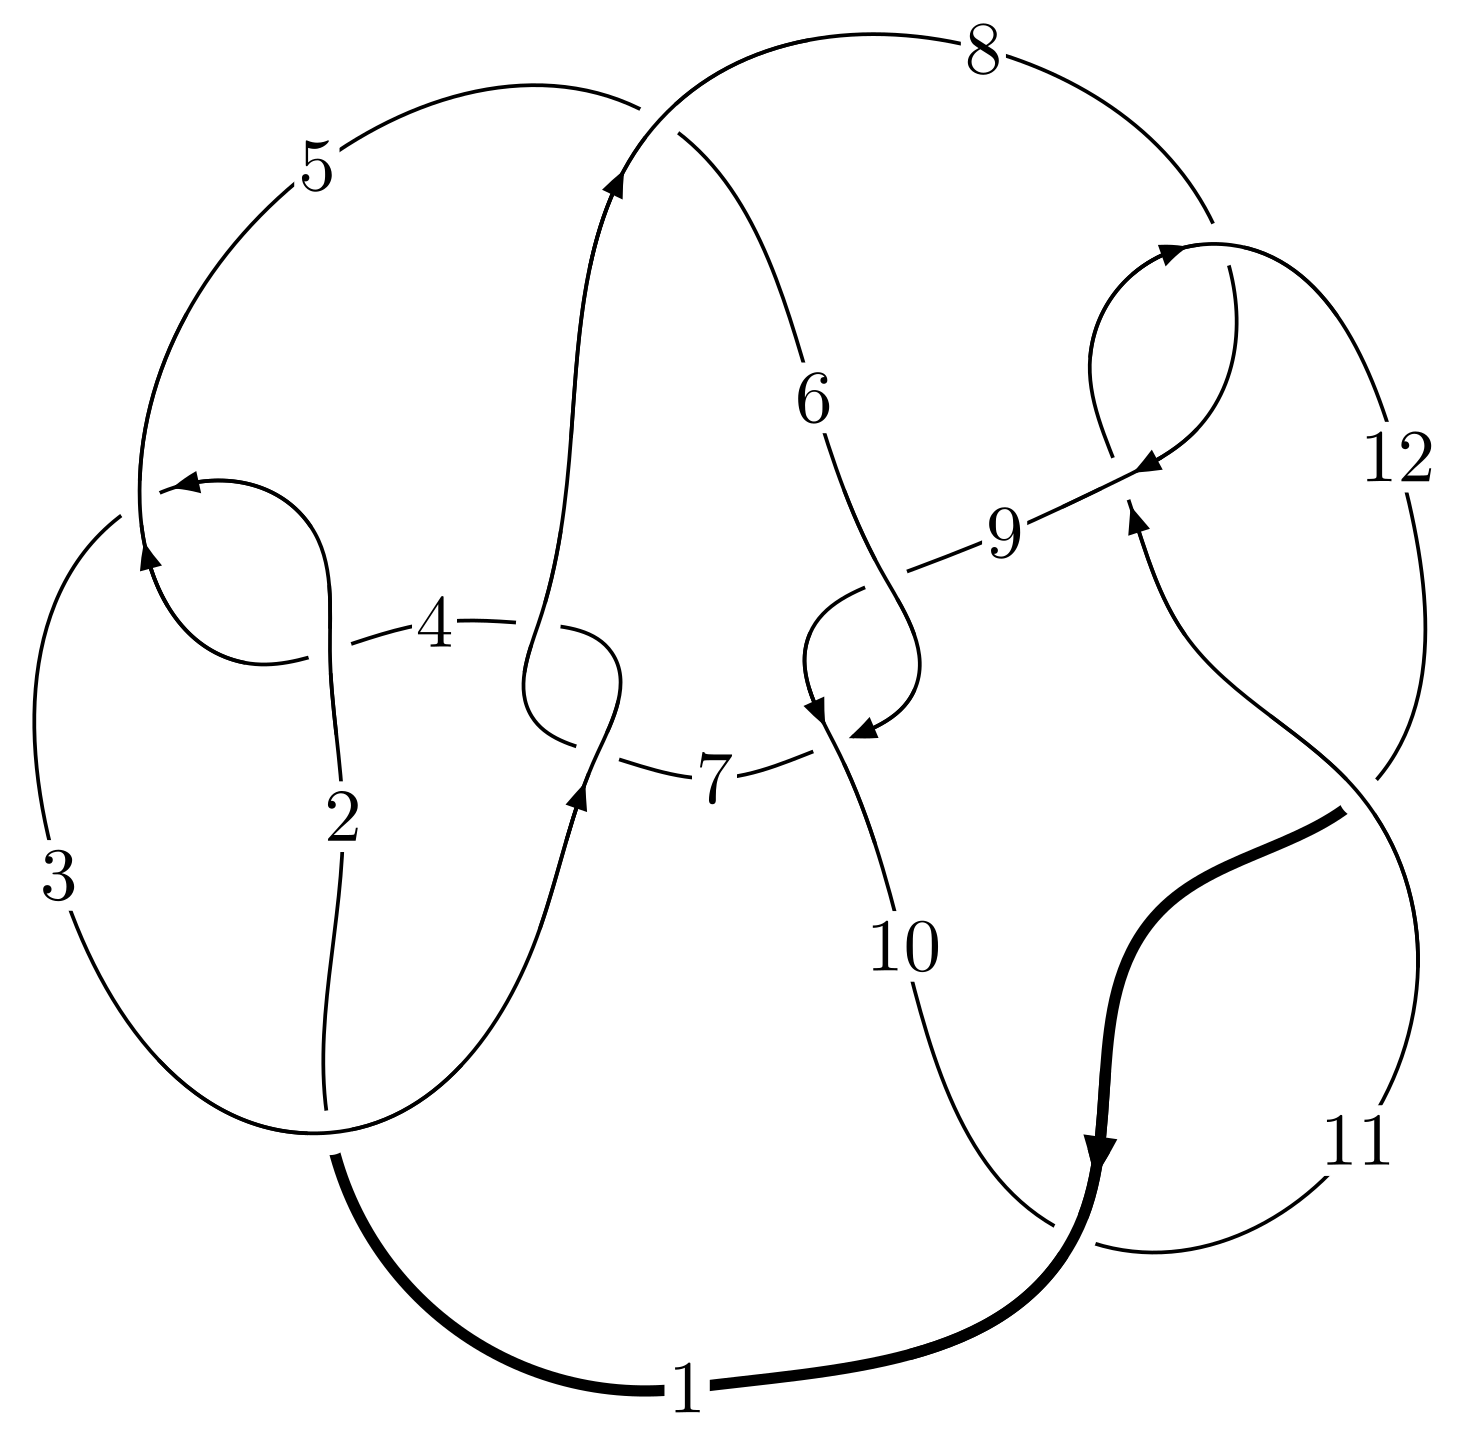
\includegraphics[width=112pt]{../../../GIT/diagram.site/Diagrams/png/2158_12n_0069.png}\\
\ \ \ A knot diagram\footnotemark}&
\allowdisplaybreaks
\textbf{Linearized knot diagam} \\
\cline{2-2}
 &
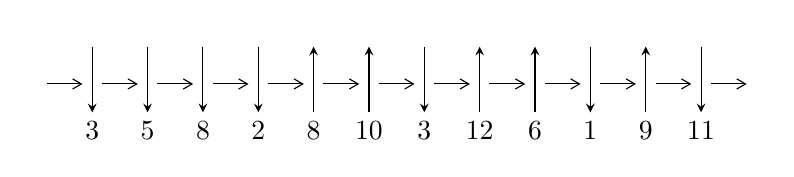
\begin{tikzpicture}[x=20pt, y=17pt]
	% nodes
	\node (C0) at (0, 0) {};
	\node (C1) at (1, 0) {};
	\node (C1U) at (1, +1) {};
	\node (C1D) at (1, -1) {3};

	\node (C2) at (2, 0) {};
	\node (C2U) at (2, +1) {};
	\node (C2D) at (2, -1) {5};

	\node (C3) at (3, 0) {};
	\node (C3U) at (3, +1) {};
	\node (C3D) at (3, -1) {8};

	\node (C4) at (4, 0) {};
	\node (C4U) at (4, +1) {};
	\node (C4D) at (4, -1) {2};

	\node (C5) at (5, 0) {};
	\node (C5U) at (5, +1) {};
	\node (C5D) at (5, -1) {8};

	\node (C6) at (6, 0) {};
	\node (C6U) at (6, +1) {};
	\node (C6D) at (6, -1) {10};

	\node (C7) at (7, 0) {};
	\node (C7U) at (7, +1) {};
	\node (C7D) at (7, -1) {3};

	\node (C8) at (8, 0) {};
	\node (C8U) at (8, +1) {};
	\node (C8D) at (8, -1) {12};

	\node (C9) at (9, 0) {};
	\node (C9U) at (9, +1) {};
	\node (C9D) at (9, -1) {6};

	\node (C10) at (10, 0) {};
	\node (C10U) at (10, +1) {};
	\node (C10D) at (10, -1) {1};

	\node (C11) at (11, 0) {};
	\node (C11U) at (11, +1) {};
	\node (C11D) at (11, -1) {9};

	\node (C12) at (12, 0) {};
	\node (C12U) at (12, +1) {};
	\node (C12D) at (12, -1) {11};
	\node (C13) at (13, 0) {};

	% arrows
	\draw[->,>={angle 60}]
	(C0) edge (C1) (C1) edge (C2) (C2) edge (C3) (C3) edge (C4) (C4) edge (C5) (C5) edge (C6) (C6) edge (C7) (C7) edge (C8) (C8) edge (C9) (C9) edge (C10) (C10) edge (C11) (C11) edge (C12) (C12) edge (C13) ;	\draw[->,>=stealth]
	(C1U) edge (C1D) (C2U) edge (C2D) (C3U) edge (C3D) (C4U) edge (C4D) (C5D) edge (C5U) (C6D) edge (C6U) (C7U) edge (C7D) (C8D) edge (C8U) (C9D) edge (C9U) (C10U) edge (C10D) (C11D) edge (C11U) (C12U) edge (C12D) ;
	\end{tikzpicture} \\
\hhline{~~} \\& 
\textbf{Solving Sequence} \\ \cline{2-2} 
 &
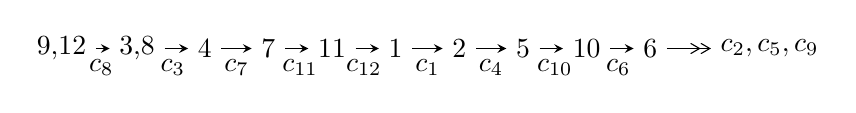
\begin{tikzpicture}[x=23pt, y=7pt]
	% node
	\node (A0) at (-1/8, 0) {9,12};
	\node (A1) at (17/16, 0) {3,8};
	\node (A2) at (17/8, 0) {4};
	\node (A3) at (25/8, 0) {7};
	\node (A4) at (33/8, 0) {11};
	\node (A5) at (41/8, 0) {1};
	\node (A6) at (49/8, 0) {2};
	\node (A7) at (57/8, 0) {5};
	\node (A8) at (65/8, 0) {10};
	\node (A9) at (73/8, 0) {6};
	\node (C1) at (1/2, -1) {$c_{8}$};
	\node (C2) at (13/8, -1) {$c_{3}$};
	\node (C3) at (21/8, -1) {$c_{7}$};
	\node (C4) at (29/8, -1) {$c_{11}$};
	\node (C5) at (37/8, -1) {$c_{12}$};
	\node (C6) at (45/8, -1) {$c_{1}$};
	\node (C7) at (53/8, -1) {$c_{4}$};
	\node (C8) at (61/8, -1) {$c_{10}$};
	\node (C9) at (69/8, -1) {$c_{6}$};
	\node (A10) at (11, 0) {$c_{2},c_{5},c_{9}$};

	% edge
	\draw[->,>=stealth]	
	(A0) edge (A1) (A1) edge (A2) (A2) edge (A3) (A3) edge (A4) (A4) edge (A5) (A5) edge (A6) (A6) edge (A7) (A7) edge (A8) (A8) edge (A9) ;
	\draw[->>,>={angle 60}]	
	(A9) edge (A10);
\end{tikzpicture} \\ 

\end{tabular} \\

\footnotetext{
The image of knot diagram is generated by the software ``\textbf{Draw programme}" developed by Andrew Bartholomew(\url{http://www.layer8.co.uk/maths/draw/index.htm\#Running-draw}), where we modified some parts for our purpose(\url{https://github.com/CATsTAILs/LinksPainter}).
}\phantom \\ \newline 
\centering \textbf{Ideals for irreducible components\footnotemark of $X_{\text{par}}$} 
 
\begin{align*}
I^u_{1}&=\langle 
-1.25022\times10^{15} u^{50}+6.32707\times10^{15} u^{49}+\cdots+5.27740\times10^{14} b+1.09741\times10^{15},\\
\phantom{I^u_{1}}&\phantom{= \langle  }-315570811462394 u^{50}+885003680032642 u^{49}+\cdots+263870210392814 a-2615309819180911,\\
\phantom{I^u_{1}}&\phantom{= \langle  }u^{51}-5 u^{50}+\cdots+12 u+1\rangle \\
I^u_{2}&=\langle 
- u^6+u^5- u^4- u^2+b,\;- u^4+u^3- u^2+a-1,\;u^9- u^8+2 u^7- u^6+3 u^5- u^4+2 u^3+u+1\rangle \\
I^u_{3}&=\langle 
- a^2 u- a u+b+u,\;a^3- a^2 u+2 a^2- a u- a+u-2,\;u^2+u+1\rangle \\
\\
\end{align*}
\raggedright * 3 irreducible components of $\dim_{\mathbb{C}}=0$, with total 66 representations.\\
\footnotetext{All coefficients of polynomials are rational numbers. But the coefficients are sometimes approximated in decimal forms when there is not enough margin.}
\newpage
\renewcommand{\arraystretch}{1}
\centering \section*{I. $I^u_{1}= \langle -1.25\times10^{15} u^{50}+6.33\times10^{15} u^{49}+\cdots+5.28\times10^{14} b+1.10\times10^{15},\;-3.16\times10^{14} u^{50}+8.85\times10^{14} u^{49}+\cdots+2.64\times10^{14} a-2.62\times10^{15},\;u^{51}-5 u^{50}+\cdots+12 u+1 \rangle$}
\flushleft \textbf{(i) Arc colorings}\\
\begin{tabular}{m{7pt} m{180pt} m{7pt} m{180pt} }
\flushright $a_{9}=$&$\begin{pmatrix}1\\0\end{pmatrix}$ \\
\flushright $a_{12}=$&$\begin{pmatrix}0\\u\end{pmatrix}$ \\
\flushright $a_{3}=$&$\begin{pmatrix}1.19593 u^{50}-3.35394 u^{49}+\cdots+22.7516 u+9.91135\\2.36901 u^{50}-11.9890 u^{49}+\cdots-33.0652 u-2.07945\end{pmatrix}$ \\
\flushright $a_{8}=$&$\begin{pmatrix}1\\u^2\end{pmatrix}$ \\
\flushright $a_{4}=$&$\begin{pmatrix}2.03208 u^{50}-6.11447 u^{49}+\cdots+23.1122 u+9.36508\\3.57786 u^{50}-18.1788 u^{49}+\cdots-50.9440 u-3.49968\end{pmatrix}$ \\
\flushright $a_{7}=$&$\begin{pmatrix}-0.655866 u^{50}+0.100505 u^{49}+\cdots-30.5833 u-5.33675\\-2.04168 u^{50}+11.1347 u^{49}+\cdots+35.7500 u+2.53294\end{pmatrix}$ \\
\flushright $a_{11}=$&$\begin{pmatrix}- u\\u\end{pmatrix}$ \\
\flushright $a_{1}=$&$\begin{pmatrix}- u^3\\u^3+u\end{pmatrix}$ \\
\flushright $a_{2}=$&$\begin{pmatrix}2.38515 u^{50}-7.53764 u^{49}+\cdots+6.70994 u+6.22567\\4.11391 u^{50}-20.5592 u^{49}+\cdots-49.6817 u-3.68437\end{pmatrix}$ \\
\flushright $a_{5}=$&$\begin{pmatrix}-0.280392 u^{50}-0.591852 u^{49}+\cdots-1.39584 u+2.65716\\-2.25255 u^{50}+11.2149 u^{49}+\cdots+29.5667 u+2.69754\end{pmatrix}$ \\
\flushright $a_{10}=$&$\begin{pmatrix}- u^5- u\\u^5+u^3+u\end{pmatrix}$ \\
\flushright $a_{6}=$&$\begin{pmatrix}0.694241 u^{50}-0.897617 u^{49}+\cdots-3.96472 u-3.36089\\2.79370 u^{50}-14.0251 u^{49}+\cdots-36.9379 u-3.27732\end{pmatrix}$\\&\end{tabular}
\flushleft \textbf{(ii) Obstruction class $= -1$}\\~\\
\flushleft \textbf{(iii) Cusp Shapes $= -\frac{255965214862211}{131935105196407} u^{50}+\frac{1522307809078135}{263870210392814} u^{49}+\cdots-\frac{2747389394610787}{131935105196407} u-\frac{1408076674646089}{131935105196407}$}\\~\\
\newpage\renewcommand{\arraystretch}{1}
\flushleft \textbf{(iv) u-Polynomials at the component}\newline \\
\begin{tabular}{m{50pt}|m{274pt}}
Crossings & \hspace{64pt}u-Polynomials at each crossing \\
\hline $$\begin{aligned}c_{1}\end{aligned}$$&$\begin{aligned}
&u^{51}+10 u^{50}+\cdots-5 u+1
\end{aligned}$\\
\hline $$\begin{aligned}c_{2},c_{4}\end{aligned}$$&$\begin{aligned}
&u^{51}-12 u^{50}+\cdots-9 u+1
\end{aligned}$\\
\hline $$\begin{aligned}c_{3},c_{7}\end{aligned}$$&$\begin{aligned}
&u^{51}-3 u^{50}+\cdots-512 u+512
\end{aligned}$\\
\hline $$\begin{aligned}c_{5}\end{aligned}$$&$\begin{aligned}
&u^{51}+4 u^{50}+\cdots- u+1
\end{aligned}$\\
\hline $$\begin{aligned}c_{6},c_{9}\end{aligned}$$&$\begin{aligned}
&u^{51}-2 u^{50}+\cdots+32 u+64
\end{aligned}$\\
\hline $$\begin{aligned}c_{8},c_{11}\end{aligned}$$&$\begin{aligned}
&u^{51}+5 u^{50}+\cdots+12 u-1
\end{aligned}$\\
\hline $$\begin{aligned}c_{10},c_{12}\end{aligned}$$&$\begin{aligned}
&u^{51}+15 u^{50}+\cdots+132 u-1
\end{aligned}$\\
\hline
\end{tabular}\\~\\
\newpage\renewcommand{\arraystretch}{1}
\flushleft \textbf{(v) Riley Polynomials at the component}\newline \\
\begin{tabular}{m{50pt}|m{274pt}}
Crossings & \hspace{64pt}Riley Polynomials at each crossing \\
\hline $$\begin{aligned}c_{1}\end{aligned}$$&$\begin{aligned}
&y^{51}+74 y^{50}+\cdots-5 y-1
\end{aligned}$\\
\hline $$\begin{aligned}c_{2},c_{4}\end{aligned}$$&$\begin{aligned}
&y^{51}-10 y^{50}+\cdots-5 y-1
\end{aligned}$\\
\hline $$\begin{aligned}c_{3},c_{7}\end{aligned}$$&$\begin{aligned}
&y^{51}+63 y^{50}+\cdots-1310720 y-262144
\end{aligned}$\\
\hline $$\begin{aligned}c_{5}\end{aligned}$$&$\begin{aligned}
&y^{51}-66 y^{50}+\cdots+55 y-1
\end{aligned}$\\
\hline $$\begin{aligned}c_{6},c_{9}\end{aligned}$$&$\begin{aligned}
&y^{51}-40 y^{50}+\cdots+33792 y-4096
\end{aligned}$\\
\hline $$\begin{aligned}c_{8},c_{11}\end{aligned}$$&$\begin{aligned}
&y^{51}+15 y^{50}+\cdots+132 y-1
\end{aligned}$\\
\hline $$\begin{aligned}c_{10},c_{12}\end{aligned}$$&$\begin{aligned}
&y^{51}+47 y^{50}+\cdots+21000 y-1
\end{aligned}$\\
\hline
\end{tabular}\\~\\
\newpage\flushleft \textbf{(vi) Complex Volumes and Cusp Shapes}
$$\begin{array}{c|c|c}  
\text{Solutions to }I^u_{1}& \I (\text{vol} + \sqrt{-1}CS) & \text{Cusp shape}\\
 \hline 
\begin{aligned}
u &= -0.536812 + 0.848543 I \\
a &= -3.28628 - 1.11420 I \\
b &= \phantom{-}0.02773 + 3.59095 I\end{aligned}
 & -1.34634 - 2.15686 I & -38.8808 - 5.4252 I \\ \hline\begin{aligned}
u &= -0.536812 - 0.848543 I \\
a &= -3.28628 + 1.11420 I \\
b &= \phantom{-}0.02773 - 3.59095 I\end{aligned}
 & -1.34634 + 2.15686 I & -38.8808 + 5.4252 I \\ \hline\begin{aligned}
u &= -0.094060 + 1.010250 I \\
a &= -0.112437 + 0.884543 I \\
b &= \phantom{-}0.240148 - 0.241280 I\end{aligned}
 & -2.30980 - 2.34904 I & -1.63391 + 4.30826 I \\ \hline\begin{aligned}
u &= -0.094060 - 1.010250 I \\
a &= -0.112437 - 0.884543 I \\
b &= \phantom{-}0.240148 + 0.241280 I\end{aligned}
 & -2.30980 + 2.34904 I & -1.63391 - 4.30826 I \\ \hline\begin{aligned}
u &= \phantom{-}0.742640 + 0.708697 I \\
a &= -0.254347 - 0.182338 I \\
b &= \phantom{-}0.276012 + 0.545830 I\end{aligned}
 & \phantom{-}3.40321 - 2.16441 I & \phantom{-}5.02879 + 4.36220 I \\ \hline\begin{aligned}
u &= \phantom{-}0.742640 - 0.708697 I \\
a &= -0.254347 + 0.182338 I \\
b &= \phantom{-}0.276012 - 0.545830 I\end{aligned}
 & \phantom{-}3.40321 + 2.16441 I & \phantom{-}5.02879 - 4.36220 I \\ \hline\begin{aligned}
u &= -0.671229 + 0.780928 I \\
a &= -0.409812 - 0.918047 I \\
b &= -0.370682 + 1.062140 I\end{aligned}
 & \phantom{-}1.10678 - 2.18307 I & \phantom{-}1.75585 + 4.26435 I \\ \hline\begin{aligned}
u &= -0.671229 - 0.780928 I \\
a &= -0.409812 + 0.918047 I \\
b &= -0.370682 - 1.062140 I\end{aligned}
 & \phantom{-}1.10678 + 2.18307 I & \phantom{-}1.75585 - 4.26435 I \\ \hline\begin{aligned}
u &= -0.343157 + 0.972562 I \\
a &= -1.52133 + 0.33833 I \\
b &= \phantom{-}0.746603 + 0.561119 I\end{aligned}
 & -0.84537 - 2.80643 I & \phantom{-}0.19319 + 7.33231 I \\ \hline\begin{aligned}
u &= -0.343157 - 0.972562 I \\
a &= -1.52133 - 0.33833 I \\
b &= \phantom{-}0.746603 - 0.561119 I\end{aligned}
 & -0.84537 + 2.80643 I & \phantom{-}0.19319 - 7.33231 I\\
 \hline 
 \end{array}$$\newpage$$\begin{array}{c|c|c}  
\text{Solutions to }I^u_{1}& \I (\text{vol} + \sqrt{-1}CS) & \text{Cusp shape}\\
 \hline 
\begin{aligned}
u &= -0.906899 + 0.049738 I \\
a &= -0.05164 + 1.55010 I \\
b &= -0.207366 - 0.576620 I\end{aligned}
 & \phantom{-}10.08960 - 3.82704 I & \phantom{-}3.71077 + 2.41179 I \\ \hline\begin{aligned}
u &= -0.906899 - 0.049738 I \\
a &= -0.05164 - 1.55010 I \\
b &= -0.207366 + 0.576620 I\end{aligned}
 & \phantom{-}10.08960 + 3.82704 I & \phantom{-}3.71077 - 2.41179 I \\ \hline\begin{aligned}
u &= -0.634734 + 0.940518 I \\
a &= -1.031740 - 0.008845 I \\
b &= \phantom{-}0.734442 + 0.646858 I\end{aligned}
 & \phantom{-}0.59171 - 2.88116 I & \phantom{-}1.02571 + 2.36792 I \\ \hline\begin{aligned}
u &= -0.634734 - 0.940518 I \\
a &= -1.031740 + 0.008845 I \\
b &= \phantom{-}0.734442 - 0.646858 I\end{aligned}
 & \phantom{-}0.59171 + 2.88116 I & \phantom{-}1.02571 - 2.36792 I \\ \hline\begin{aligned}
u &= -0.231781 + 0.820128 I \\
a &= \phantom{-}1.19571 + 1.76809 I \\
b &= \phantom{-}0.08039 - 2.15413 I\end{aligned}
 & -2.70466 - 1.62087 I & -0.49766 + 1.58102 I \\ \hline\begin{aligned}
u &= -0.231781 - 0.820128 I \\
a &= \phantom{-}1.19571 - 1.76809 I \\
b &= \phantom{-}0.08039 + 2.15413 I\end{aligned}
 & -2.70466 + 1.62087 I & -0.49766 - 1.58102 I \\ \hline\begin{aligned}
u &= \phantom{-}0.281941 + 0.765767 I \\
a &= \phantom{-}2.01085 + 0.32244 I \\
b &= -0.827511 - 0.669898 I\end{aligned}
 & \phantom{-}2.53081 + 4.23664 I & -4.52353 + 0.13902 I \\ \hline\begin{aligned}
u &= \phantom{-}0.281941 - 0.765767 I \\
a &= \phantom{-}2.01085 - 0.32244 I \\
b &= -0.827511 + 0.669898 I\end{aligned}
 & \phantom{-}2.53081 - 4.23664 I & -4.52353 - 0.13902 I \\ \hline\begin{aligned}
u &= \phantom{-}0.946253 + 0.718970 I \\
a &= \phantom{-}0.29613 + 1.52046 I \\
b &= -2.57630 - 0.83741 I\end{aligned}
 & \phantom{-}14.2145 - 8.1932 I & \phantom{-}2.56257 + 3.05589 I \\ \hline\begin{aligned}
u &= \phantom{-}0.946253 - 0.718970 I \\
a &= \phantom{-}0.29613 - 1.52046 I \\
b &= -2.57630 + 0.83741 I\end{aligned}
 & \phantom{-}14.2145 + 8.1932 I & \phantom{-}2.56257 - 3.05589 I\\
 \hline 
 \end{array}$$\newpage$$\begin{array}{c|c|c}  
\text{Solutions to }I^u_{1}& \I (\text{vol} + \sqrt{-1}CS) & \text{Cusp shape}\\
 \hline 
\begin{aligned}
u &= \phantom{-}0.818205 + 0.870861 I \\
a &= \phantom{-}0.71161 + 1.65346 I \\
b &= -1.57668 - 0.05628 I\end{aligned}
 & \phantom{-}3.54064 + 1.51067 I & \phantom{-0.000000 } 0. - 2.09785 I \\ \hline\begin{aligned}
u &= \phantom{-}0.818205 - 0.870861 I \\
a &= \phantom{-}0.71161 - 1.65346 I \\
b &= -1.57668 + 0.05628 I\end{aligned}
 & \phantom{-}3.54064 - 1.51067 I & \phantom{-0.000000 -}0. + 2.09785 I \\ \hline\begin{aligned}
u &= \phantom{-}0.869595 + 0.828375 I \\
a &= \phantom{-}0.627708 + 0.017566 I \\
b &= -1.261280 + 0.334121 I\end{aligned}
 & \phantom{-}7.00223 - 0.65691 I & \phantom{-}3.27323 + 0. I\phantom{ +0.000000I} \\ \hline\begin{aligned}
u &= \phantom{-}0.869595 - 0.828375 I \\
a &= \phantom{-}0.627708 - 0.017566 I \\
b &= -1.261280 - 0.334121 I\end{aligned}
 & \phantom{-}7.00223 + 0.65691 I & \phantom{-}3.27323 + 0. I\phantom{ +0.000000I} \\ \hline\begin{aligned}
u &= \phantom{-}0.703781 + 0.984612 I \\
a &= \phantom{-}0.766481 + 0.030963 I \\
b &= -0.309574 + 0.323070 I\end{aligned}
 & \phantom{-}2.57944 + 7.69347 I & \phantom{-}4.07652 - 9.82403 I \\ \hline\begin{aligned}
u &= \phantom{-}0.703781 - 0.984612 I \\
a &= \phantom{-}0.766481 - 0.030963 I \\
b &= -0.309574 - 0.323070 I\end{aligned}
 & \phantom{-}2.57944 - 7.69347 I & \phantom{-}4.07652 + 9.82403 I \\ \hline\begin{aligned}
u &= -0.839716 + 0.871954 I \\
a &= -1.06327 + 2.00567 I \\
b &= \phantom{-}3.24142 - 0.39313 I\end{aligned}
 & \phantom{-}9.25314 + 0.69544 I & \phantom{-0.000000 } 0 \\ \hline\begin{aligned}
u &= -0.839716 - 0.871954 I \\
a &= -1.06327 - 2.00567 I \\
b &= \phantom{-}3.24142 + 0.39313 I\end{aligned}
 & \phantom{-}9.25314 - 0.69544 I & \phantom{-0.000000 } 0 \\ \hline\begin{aligned}
u &= -0.277519 + 1.189370 I \\
a &= -1.44184 - 0.41933 I \\
b &= \phantom{-}1.239660 - 0.206290 I\end{aligned}
 & \phantom{-}5.79395 - 7.83565 I & \phantom{-0.000000 -}0. + 5.73327 I \\ \hline\begin{aligned}
u &= -0.277519 - 1.189370 I \\
a &= -1.44184 + 0.41933 I \\
b &= \phantom{-}1.239660 + 0.206290 I\end{aligned}
 & \phantom{-}5.79395 + 7.83565 I & \phantom{-0.000000 } 0. - 5.73327 I\\
 \hline 
 \end{array}$$\newpage$$\begin{array}{c|c|c}  
\text{Solutions to }I^u_{1}& \I (\text{vol} + \sqrt{-1}CS) & \text{Cusp shape}\\
 \hline 
\begin{aligned}
u &= \phantom{-}0.803600 + 0.919882 I \\
a &= -0.473301 - 0.798618 I \\
b &= \phantom{-}1.99513 + 0.47998 I\end{aligned}
 & \phantom{-}3.38835 + 4.55859 I & \phantom{-0.000000 } 0. - 3.21833 I \\ \hline\begin{aligned}
u &= \phantom{-}0.803600 - 0.919882 I \\
a &= -0.473301 + 0.798618 I \\
b &= \phantom{-}1.99513 - 0.47998 I\end{aligned}
 & \phantom{-}3.38835 - 4.55859 I & \phantom{-0.000000 -}0. + 3.21833 I \\ \hline\begin{aligned}
u &= \phantom{-}0.951705 + 0.774303 I \\
a &= -0.44896 - 1.74202 I \\
b &= \phantom{-}2.48425 + 0.81897 I\end{aligned}
 & \phantom{-}15.3068 - 0.2972 I & \phantom{-0.000000 } 0 \\ \hline\begin{aligned}
u &= \phantom{-}0.951705 - 0.774303 I \\
a &= -0.44896 + 1.74202 I \\
b &= \phantom{-}2.48425 - 0.81897 I\end{aligned}
 & \phantom{-}15.3068 + 0.2972 I & \phantom{-0.000000 } 0 \\ \hline\begin{aligned}
u &= -0.348613 + 1.179410 I \\
a &= \phantom{-}0.874337 + 0.615537 I \\
b &= -0.753430 + 0.266431 I\end{aligned}
 & \phantom{-}6.24476 - 0.53865 I & \phantom{-0.000000 } 0 \\ \hline\begin{aligned}
u &= -0.348613 - 1.179410 I \\
a &= \phantom{-}0.874337 - 0.615537 I \\
b &= -0.753430 - 0.266431 I\end{aligned}
 & \phantom{-}6.24476 + 0.53865 I & \phantom{-0.000000 } 0 \\ \hline\begin{aligned}
u &= -0.817892 + 0.928643 I \\
a &= \phantom{-}1.28285 - 2.22579 I \\
b &= -3.27673 + 0.29519 I\end{aligned}
 & \phantom{-}9.07395 - 6.87436 I & \phantom{-0.000000 -}0. + 4.69588 I \\ \hline\begin{aligned}
u &= -0.817892 - 0.928643 I \\
a &= \phantom{-}1.28285 + 2.22579 I \\
b &= -3.27673 - 0.29519 I\end{aligned}
 & \phantom{-}9.07395 + 6.87436 I & \phantom{-0.000000 } 0. - 4.69588 I \\ \hline\begin{aligned}
u &= \phantom{-}0.815253 + 0.972044 I \\
a &= -0.129107 - 1.389170 I \\
b &= \phantom{-}0.894314 + 0.620552 I\end{aligned}
 & \phantom{-}6.55249 + 6.91504 I & \phantom{-0.000000 } 0 \\ \hline\begin{aligned}
u &= \phantom{-}0.815253 - 0.972044 I \\
a &= -0.129107 + 1.389170 I \\
b &= \phantom{-}0.894314 - 0.620552 I\end{aligned}
 & \phantom{-}6.55249 - 6.91504 I & \phantom{-0.000000 } 0\\
 \hline 
 \end{array}$$\newpage$$\begin{array}{c|c|c}  
\text{Solutions to }I^u_{1}& \I (\text{vol} + \sqrt{-1}CS) & \text{Cusp shape}\\
 \hline 
\begin{aligned}
u &= \phantom{-}0.382213 + 0.598227 I \\
a &= -1.50501 - 0.47756 I \\
b &= \phantom{-}0.588819 + 0.737449 I\end{aligned}
 & \phantom{-}3.06808 - 1.61207 I & -0.16491 + 5.64429 I \\ \hline\begin{aligned}
u &= \phantom{-}0.382213 - 0.598227 I \\
a &= -1.50501 + 0.47756 I \\
b &= \phantom{-}0.588819 - 0.737449 I\end{aligned}
 & \phantom{-}3.06808 + 1.61207 I & -0.16491 - 5.64429 I \\ \hline\begin{aligned}
u &= \phantom{-}0.793119 + 1.061710 I \\
a &= -1.78595 - 1.61228 I \\
b &= \phantom{-}2.94405 - 0.44989 I\end{aligned}
 & \phantom{-}13.1325 + 14.5878 I & \phantom{-0.000000 } 0 \\ \hline\begin{aligned}
u &= \phantom{-}0.793119 - 1.061710 I \\
a &= -1.78595 + 1.61228 I \\
b &= \phantom{-}2.94405 + 0.44989 I\end{aligned}
 & \phantom{-}13.1325 - 14.5878 I & \phantom{-0.000000 } 0 \\ \hline\begin{aligned}
u &= \phantom{-}0.827403 + 1.041820 I \\
a &= \phantom{-}1.65771 + 1.36481 I \\
b &= -2.86877 + 0.33442 I\end{aligned}
 & \phantom{-}14.4581 + 6.8314 I & \phantom{-0.000000 } 0 \\ \hline\begin{aligned}
u &= \phantom{-}0.827403 - 1.041820 I \\
a &= \phantom{-}1.65771 - 1.36481 I \\
b &= -2.86877 - 0.33442 I\end{aligned}
 & \phantom{-}14.4581 - 6.8314 I & \phantom{-0.000000 } 0 \\ \hline\begin{aligned}
u &= -0.105235 + 0.624758 I \\
a &= \phantom{-}1.54589 + 1.13818 I \\
b &= \phantom{-}0.324601 - 0.482306 I\end{aligned}
 & -1.65146 - 0.02846 I & -5.98427 + 0.19920 I \\ \hline\begin{aligned}
u &= -0.105235 - 0.624758 I \\
a &= \phantom{-}1.54589 - 1.13818 I \\
b &= \phantom{-}0.324601 + 0.482306 I\end{aligned}
 & -1.65146 + 0.02846 I & -5.98427 - 0.19920 I \\ \hline\begin{aligned}
u &= -0.586526 + 0.208462 I \\
a &= -0.208700 - 0.246043 I \\
b &= -0.565071 + 0.589283 I\end{aligned}
 & \phantom{-}1.50163 - 0.56025 I & \phantom{-}5.46794 + 1.34072 I \\ \hline\begin{aligned}
u &= -0.586526 - 0.208462 I \\
a &= -0.208700 + 0.246043 I \\
b &= -0.565071 - 0.589283 I\end{aligned}
 & \phantom{-}1.50163 + 0.56025 I & \phantom{-}5.46794 - 1.34072 I\\
 \hline 
 \end{array}$$\newpage$$\begin{array}{c|c|c}  
\text{Solutions to }I^u_{1}& \I (\text{vol} + \sqrt{-1}CS) & \text{Cusp shape}\\
 \hline 
\begin{aligned}
u &= -0.0830715\phantom{ +0.000000I} \\
a &= \phantom{-}8.50895\phantom{ +0.000000I} \\
b &= \phantom{-}0.551653\phantom{ +0.000000I}\end{aligned}
 & -1.20993\phantom{ +0.000000I} & -9.33730\phantom{ +0.000000I}\\
 \hline 
 \end{array}$$\newpage\newpage\renewcommand{\arraystretch}{1}
\centering \section*{II. $I^u_{2}= \langle - u^6+u^5- u^4- u^2+b,\;- u^4+u^3- u^2+a-1,\;u^9- u^8+2 u^7- u^6+3 u^5- u^4+2 u^3+u+1 \rangle$}
\flushleft \textbf{(i) Arc colorings}\\
\begin{tabular}{m{7pt} m{180pt} m{7pt} m{180pt} }
\flushright $a_{9}=$&$\begin{pmatrix}1\\0\end{pmatrix}$ \\
\flushright $a_{12}=$&$\begin{pmatrix}0\\u\end{pmatrix}$ \\
\flushright $a_{3}=$&$\begin{pmatrix}u^4- u^3+u^2+1\\u^6- u^5+u^4+u^2\end{pmatrix}$ \\
\flushright $a_{8}=$&$\begin{pmatrix}1\\u^2\end{pmatrix}$ \\
\flushright $a_{4}=$&$\begin{pmatrix}u^4- u^3+u^2+1\\u^6- u^5+u^4+u^2\end{pmatrix}$ \\
\flushright $a_{7}=$&$\begin{pmatrix}1\\u^2\end{pmatrix}$ \\
\flushright $a_{11}=$&$\begin{pmatrix}- u\\u\end{pmatrix}$ \\
\flushright $a_{1}=$&$\begin{pmatrix}- u^3\\u^3+u\end{pmatrix}$ \\
\flushright $a_{2}=$&$\begin{pmatrix}u^4-2 u^3+u^2+1\\u^6- u^5+u^4+u^3+u^2+u\end{pmatrix}$ \\
\flushright $a_{5}=$&$\begin{pmatrix}u^3\\- u^3- u\end{pmatrix}$ \\
\flushright $a_{10}=$&$\begin{pmatrix}- u^5- u\\u^5+u^3+u\end{pmatrix}$ \\
\flushright $a_{6}=$&$\begin{pmatrix}- u^5- u\\- u^7- u^5-2 u^3- u\end{pmatrix}$\\&\end{tabular}
\flushleft \textbf{(ii) Obstruction class $= 1$}\\~\\
\flushleft \textbf{(iii) Cusp Shapes $= 2 u^8-7 u^7+8 u^6-8 u^5+8 u^4-12 u^3+6 u^2-2 u-2$}\\~\\
\newpage\renewcommand{\arraystretch}{1}
\flushleft \textbf{(iv) u-Polynomials at the component}\newline \\
\begin{tabular}{m{50pt}|m{274pt}}
Crossings & \hspace{64pt}u-Polynomials at each crossing \\
\hline $$\begin{aligned}c_{1},c_{2}\end{aligned}$$&$\begin{aligned}
&(u-1)^9
\end{aligned}$\\
\hline $$\begin{aligned}c_{3},c_{7}\end{aligned}$$&$\begin{aligned}
&u^9
\end{aligned}$\\
\hline $$\begin{aligned}c_{4}\end{aligned}$$&$\begin{aligned}
&(u+1)^9
\end{aligned}$\\
\hline $$\begin{aligned}c_{5}\end{aligned}$$&$\begin{aligned}
&u^9+5 u^8+12 u^7+15 u^6+9 u^5- u^4-4 u^3-2 u^2+u+1
\end{aligned}$\\
\hline $$\begin{aligned}c_{6}\end{aligned}$$&$\begin{aligned}
&u^9- u^8-2 u^7+3 u^6+u^5-3 u^4+2 u^3- u+1
\end{aligned}$\\
\hline $$\begin{aligned}c_{8}\end{aligned}$$&$\begin{aligned}
&u^9- u^8+2 u^7- u^6+3 u^5- u^4+2 u^3+u+1
\end{aligned}$\\
\hline $$\begin{aligned}c_{9}\end{aligned}$$&$\begin{aligned}
&u^9+u^8-2 u^7-3 u^6+u^5+3 u^4+2 u^3- u-1
\end{aligned}$\\
\hline $$\begin{aligned}c_{10}\end{aligned}$$&$\begin{aligned}
&u^9-3 u^8+8 u^7-13 u^6+17 u^5-17 u^4+12 u^3-6 u^2+u+1
\end{aligned}$\\
\hline $$\begin{aligned}c_{11}\end{aligned}$$&$\begin{aligned}
&u^9+u^8+2 u^7+u^6+3 u^5+u^4+2 u^3+u-1
\end{aligned}$\\
\hline $$\begin{aligned}c_{12}\end{aligned}$$&$\begin{aligned}
&u^9+3 u^8+8 u^7+13 u^6+17 u^5+17 u^4+12 u^3+6 u^2+u-1
\end{aligned}$\\
\hline
\end{tabular}\\~\\
\newpage\renewcommand{\arraystretch}{1}
\flushleft \textbf{(v) Riley Polynomials at the component}\newline \\
\begin{tabular}{m{50pt}|m{274pt}}
Crossings & \hspace{64pt}Riley Polynomials at each crossing \\
\hline $$\begin{aligned}c_{1},c_{2},c_{4}\end{aligned}$$&$\begin{aligned}
&(y-1)^9
\end{aligned}$\\
\hline $$\begin{aligned}c_{3},c_{7}\end{aligned}$$&$\begin{aligned}
&y^9
\end{aligned}$\\
\hline $$\begin{aligned}c_{5}\end{aligned}$$&$\begin{aligned}
&y^9- y^8+12 y^7-7 y^6+37 y^5+y^4-10 y^2+5 y-1
\end{aligned}$\\
\hline $$\begin{aligned}c_{6},c_{9}\end{aligned}$$&$\begin{aligned}
&y^9-5 y^8+12 y^7-15 y^6+9 y^5+y^4-4 y^3+2 y^2+y-1
\end{aligned}$\\
\hline $$\begin{aligned}c_{8},c_{11}\end{aligned}$$&$\begin{aligned}
&y^9+3 y^8+8 y^7+13 y^6+17 y^5+17 y^4+12 y^3+6 y^2+y-1
\end{aligned}$\\
\hline $$\begin{aligned}c_{10},c_{12}\end{aligned}$$&$\begin{aligned}
&y^9+7 y^8+20 y^7+25 y^6+5 y^5-15 y^4+22 y^2+13 y-1
\end{aligned}$\\
\hline
\end{tabular}\\~\\
\newpage\flushleft \textbf{(vi) Complex Volumes and Cusp Shapes}
$$\begin{array}{c|c|c}  
\text{Solutions to }I^u_{2}& \I (\text{vol} + \sqrt{-1}CS) & \text{Cusp shape}\\
 \hline 
\begin{aligned}
u &= -0.140343 + 0.966856 I \\
a &= \phantom{-}0.457852 + 1.072010 I \\
b &= -0.128062 - 1.105260 I\end{aligned}
 & -3.42837 - 2.09337 I & -9.96342 + 4.61282 I \\ \hline\begin{aligned}
u &= -0.140343 - 0.966856 I \\
a &= \phantom{-}0.457852 - 1.072010 I \\
b &= -0.128062 + 1.105260 I\end{aligned}
 & -3.42837 + 2.09337 I & -9.96342 - 4.61282 I \\ \hline\begin{aligned}
u &= -0.628449 + 0.875112 I \\
a &= -1.63880 - 0.65075 I \\
b &= -0.10799 + 2.04391 I\end{aligned}
 & -1.02799 - 2.45442 I & -3.17587 + 4.82524 I \\ \hline\begin{aligned}
u &= -0.628449 - 0.875112 I \\
a &= -1.63880 + 0.65075 I \\
b &= -0.10799 - 2.04391 I\end{aligned}
 & -1.02799 + 2.45442 I & -3.17587 - 4.82524 I \\ \hline\begin{aligned}
u &= \phantom{-}0.796005 + 0.733148 I \\
a &= \phantom{-}0.522253 + 0.392004 I \\
b &= -0.407341 + 0.647242 I\end{aligned}
 & \phantom{-}2.72642 - 1.33617 I & \phantom{-}0.058077 - 1.140630 I \\ \hline\begin{aligned}
u &= \phantom{-}0.796005 - 0.733148 I \\
a &= \phantom{-}0.522253 - 0.392004 I \\
b &= -0.407341 - 0.647242 I\end{aligned}
 & \phantom{-}2.72642 + 1.33617 I & \phantom{-}0.058077 + 1.140630 I \\ \hline\begin{aligned}
u &= \phantom{-}0.728966 + 0.986295 I \\
a &= \phantom{-}0.425734 - 0.444312 I \\
b &= \phantom{-}0.450985 + 0.808297 I\end{aligned}
 & \phantom{-}1.95319 + 7.08493 I & -2.55209 - 3.65320 I \\ \hline\begin{aligned}
u &= \phantom{-}0.728966 - 0.986295 I \\
a &= \phantom{-}0.425734 + 0.444312 I \\
b &= \phantom{-}0.450985 - 0.808297 I\end{aligned}
 & \phantom{-}1.95319 - 7.08493 I & -2.55209 + 3.65320 I \\ \hline\begin{aligned}
u &= -0.512358\phantom{ +0.000000I} \\
a &= \phantom{-}1.46592\phantom{ +0.000000I} \\
b &= \phantom{-}0.384820\phantom{ +0.000000I}\end{aligned}
 & -0.446489\phantom{ +0.000000I} & \phantom{-}3.26660\phantom{ +0.000000I}\\
 \hline 
 \end{array}$$\newpage\newpage\renewcommand{\arraystretch}{1}
\centering \section*{III. $I^u_{3}= \langle - a^2 u- a u+b+u,\;a^3- a^2 u+2 a^2- a u- a+u-2,\;u^2+u+1 \rangle$}
\flushleft \textbf{(i) Arc colorings}\\
\begin{tabular}{m{7pt} m{180pt} m{7pt} m{180pt} }
\flushright $a_{9}=$&$\begin{pmatrix}1\\0\end{pmatrix}$ \\
\flushright $a_{12}=$&$\begin{pmatrix}0\\u\end{pmatrix}$ \\
\flushright $a_{3}=$&$\begin{pmatrix}a\\a^2 u+a u- u\end{pmatrix}$ \\
\flushright $a_{8}=$&$\begin{pmatrix}1\\- u-1\end{pmatrix}$ \\
\flushright $a_{4}=$&$\begin{pmatrix}- a^2 u-2 a u+u\\a^2 u- a^2+2 a u- a- u+1\end{pmatrix}$ \\
\flushright $a_{7}=$&$\begin{pmatrix}a^2 u+a u+a-3 u\\0\end{pmatrix}$ \\
\flushright $a_{11}=$&$\begin{pmatrix}- u\\u\end{pmatrix}$ \\
\flushright $a_{1}=$&$\begin{pmatrix}-1\\u+1\end{pmatrix}$ \\
\flushright $a_{2}=$&$\begin{pmatrix}a^2 u+a u+a-3 u-2\\2 u+2\end{pmatrix}$ \\
\flushright $a_{5}=$&$\begin{pmatrix}a^2 u+a^2+a-3 u-3\\- a^2 u- a^2- a+3 u+3\end{pmatrix}$ \\
\flushright $a_{10}=$&$\begin{pmatrix}1\\0\end{pmatrix}$ \\
\flushright $a_{6}=$&$\begin{pmatrix}a^2 u+a u+a-3 u\\0\end{pmatrix}$\\&\end{tabular}
\flushleft \textbf{(ii) Obstruction class $= 1$}\\~\\
\flushleft \textbf{(iii) Cusp Shapes $= -8 a^2 u-4 a^2-6 a u-7 a+16 u+9$}\\~\\
\newpage\renewcommand{\arraystretch}{1}
\flushleft \textbf{(iv) u-Polynomials at the component}\newline \\
\begin{tabular}{m{50pt}|m{274pt}}
Crossings & \hspace{64pt}u-Polynomials at each crossing \\
\hline $$\begin{aligned}c_{1},c_{3}\end{aligned}$$&$\begin{aligned}
&(u^3- u^2+2 u-1)^2
\end{aligned}$\\
\hline $$\begin{aligned}c_{2}\end{aligned}$$&$\begin{aligned}
&(u^3+u^2-1)^2
\end{aligned}$\\
\hline $$\begin{aligned}c_{4}\end{aligned}$$&$\begin{aligned}
&(u^3- u^2+1)^2
\end{aligned}$\\
\hline $$\begin{aligned}c_{5}\end{aligned}$$&$\begin{aligned}
&(u^3+3 u^2+2 u-1)^2
\end{aligned}$\\
\hline $$\begin{aligned}c_{6},c_{9}\end{aligned}$$&$\begin{aligned}
&u^6
\end{aligned}$\\
\hline $$\begin{aligned}c_{7}\end{aligned}$$&$\begin{aligned}
&(u^3+u^2+2 u+1)^2
\end{aligned}$\\
\hline $$\begin{aligned}c_{8},c_{12}\end{aligned}$$&$\begin{aligned}
&(u^2+u+1)^3
\end{aligned}$\\
\hline $$\begin{aligned}c_{10},c_{11}\end{aligned}$$&$\begin{aligned}
&(u^2- u+1)^3
\end{aligned}$\\
\hline
\end{tabular}\\~\\
\newpage\renewcommand{\arraystretch}{1}
\flushleft \textbf{(v) Riley Polynomials at the component}\newline \\
\begin{tabular}{m{50pt}|m{274pt}}
Crossings & \hspace{64pt}Riley Polynomials at each crossing \\
\hline $$\begin{aligned}c_{1},c_{3},c_{7}\end{aligned}$$&$\begin{aligned}
&(y^3+3 y^2+2 y-1)^2
\end{aligned}$\\
\hline $$\begin{aligned}c_{2},c_{4}\end{aligned}$$&$\begin{aligned}
&(y^3- y^2+2 y-1)^2
\end{aligned}$\\
\hline $$\begin{aligned}c_{5}\end{aligned}$$&$\begin{aligned}
&(y^3-5 y^2+10 y-1)^2
\end{aligned}$\\
\hline $$\begin{aligned}c_{6},c_{9}\end{aligned}$$&$\begin{aligned}
&y^6
\end{aligned}$\\
\hline $$\begin{aligned}c_{8},c_{10},c_{11}\\c_{12}\end{aligned}$$&$\begin{aligned}
&(y^2+y+1)^3
\end{aligned}$\\
\hline
\end{tabular}\\~\\
\newpage\flushleft \textbf{(vi) Complex Volumes and Cusp Shapes}
$$\begin{array}{c|c|c}  
\text{Solutions to }I^u_{3}& \I (\text{vol} + \sqrt{-1}CS) & \text{Cusp shape}\\
 \hline 
\begin{aligned}
u &= -0.500000 + 0.866025 I \\
a &= \phantom{-}0.901916 + 0.094973 I \\
b &= -0.583789 + 0.478572 I\end{aligned}
 & \phantom{-}3.02413 + 0.79824 I & -0.92725 + 3.21674 I \\ \hline\begin{aligned}
u &= -0.500000 + 0.866025 I \\
a &= -1.362120 + 0.277556 I \\
b &= \phantom{-}0.706350 - 0.266290 I\end{aligned}
 & \phantom{-}3.02413 - 4.85801 I & \phantom{-}2.65209 + 7.50333 I \\ \hline\begin{aligned}
u &= -0.500000 + 0.866025 I \\
a &= -2.03980 + 0.49350 I \\
b &= \phantom{-}0.87744 + 1.51977 I\end{aligned}
 & -1.11345 - 2.02988 I & -2.22484 - 4.65789 I \\ \hline\begin{aligned}
u &= -0.500000 - 0.866025 I \\
a &= \phantom{-}0.901916 - 0.094973 I \\
b &= -0.583789 - 0.478572 I\end{aligned}
 & \phantom{-}3.02413 - 0.79824 I & -0.92725 - 3.21674 I \\ \hline\begin{aligned}
u &= -0.500000 - 0.866025 I \\
a &= -1.362120 - 0.277556 I \\
b &= \phantom{-}0.706350 + 0.266290 I\end{aligned}
 & \phantom{-}3.02413 + 4.85801 I & \phantom{-}2.65209 - 7.50333 I \\ \hline\begin{aligned}
u &= -0.500000 - 0.866025 I \\
a &= -2.03980 - 0.49350 I \\
b &= \phantom{-}0.87744 - 1.51977 I\end{aligned}
 & -1.11345 + 2.02988 I & -2.22484 + 4.65789 I\\
 \hline 
 \end{array}$$\newpage
\newpage\renewcommand{\arraystretch}{1}
\centering \section*{ IV. u-Polynomials}
\begin{tabular}{m{50pt}|m{274pt}}
Crossings & \hspace{64pt}u-Polynomials at each crossing \\
\hline $$\begin{aligned}c_{1}\end{aligned}$$&$\begin{aligned}
&((u-1)^9)(u^3- u^2+2 u-1)^2(u^{51}+10 u^{50}+\cdots-5 u+1)
\end{aligned}$\\
\hline $$\begin{aligned}c_{2}\end{aligned}$$&$\begin{aligned}
&((u-1)^9)(u^3+u^2-1)^2(u^{51}-12 u^{50}+\cdots-9 u+1)
\end{aligned}$\\
\hline $$\begin{aligned}c_{3}\end{aligned}$$&$\begin{aligned}
&u^9(u^3- u^2+2 u-1)^2(u^{51}-3 u^{50}+\cdots-512 u+512)
\end{aligned}$\\
\hline $$\begin{aligned}c_{4}\end{aligned}$$&$\begin{aligned}
&((u+1)^9)(u^3- u^2+1)^2(u^{51}-12 u^{50}+\cdots-9 u+1)
\end{aligned}$\\
\hline $$\begin{aligned}c_{5}\end{aligned}$$&$\begin{aligned}
&(u^3+3 u^2+2 u-1)^2\\
&\cdot(u^9+5 u^8+12 u^7+15 u^6+9 u^5- u^4-4 u^3-2 u^2+u+1)\\
&\cdot(u^{51}+4 u^{50}+\cdots- u+1)
\end{aligned}$\\
\hline $$\begin{aligned}c_{6}\end{aligned}$$&$\begin{aligned}
&u^6(u^9- u^8-2 u^7+3 u^6+u^5-3 u^4+2 u^3- u+1)\\
&\cdot(u^{51}-2 u^{50}+\cdots+32 u+64)
\end{aligned}$\\
\hline $$\begin{aligned}c_{7}\end{aligned}$$&$\begin{aligned}
&u^9(u^3+u^2+2 u+1)^2(u^{51}-3 u^{50}+\cdots-512 u+512)
\end{aligned}$\\
\hline $$\begin{aligned}c_{8}\end{aligned}$$&$\begin{aligned}
&(u^2+u+1)^3(u^9- u^8+2 u^7- u^6+3 u^5- u^4+2 u^3+u+1)\\
&\cdot(u^{51}+5 u^{50}+\cdots+12 u-1)
\end{aligned}$\\
\hline $$\begin{aligned}c_{9}\end{aligned}$$&$\begin{aligned}
&u^6(u^9+u^8-2 u^7-3 u^6+u^5+3 u^4+2 u^3- u-1)\\
&\cdot(u^{51}-2 u^{50}+\cdots+32 u+64)
\end{aligned}$\\
\hline $$\begin{aligned}c_{10}\end{aligned}$$&$\begin{aligned}
&(u^2- u+1)^3\\
&\cdot(u^9-3 u^8+8 u^7-13 u^6+17 u^5-17 u^4+12 u^3-6 u^2+u+1)\\
&\cdot(u^{51}+15 u^{50}+\cdots+132 u-1)
\end{aligned}$\\
\hline $$\begin{aligned}c_{11}\end{aligned}$$&$\begin{aligned}
&(u^2- u+1)^3(u^9+u^8+2 u^7+u^6+3 u^5+u^4+2 u^3+u-1)\\
&\cdot(u^{51}+5 u^{50}+\cdots+12 u-1)
\end{aligned}$\\
\hline $$\begin{aligned}c_{12}\end{aligned}$$&$\begin{aligned}
&(u^2+u+1)^3\\
&\cdot(u^9+3 u^8+8 u^7+13 u^6+17 u^5+17 u^4+12 u^3+6 u^2+u-1)\\
&\cdot(u^{51}+15 u^{50}+\cdots+132 u-1)
\end{aligned}$\\
\hline
\end{tabular}\newpage\renewcommand{\arraystretch}{1}
\centering \section*{ V. Riley Polynomials}
\begin{tabular}{m{50pt}|m{274pt}}
Crossings & \hspace{64pt}Riley Polynomials at each crossing \\
\hline $$\begin{aligned}c_{1}\end{aligned}$$&$\begin{aligned}
&((y-1)^9)(y^3+3 y^2+2 y-1)^2(y^{51}+74 y^{50}+\cdots-5 y-1)
\end{aligned}$\\
\hline $$\begin{aligned}c_{2},c_{4}\end{aligned}$$&$\begin{aligned}
&((y-1)^9)(y^3- y^2+2 y-1)^2(y^{51}-10 y^{50}+\cdots-5 y-1)
\end{aligned}$\\
\hline $$\begin{aligned}c_{3},c_{7}\end{aligned}$$&$\begin{aligned}
&y^9(y^3+3 y^2+2 y-1)^2(y^{51}+63 y^{50}+\cdots-1310720 y-262144)
\end{aligned}$\\
\hline $$\begin{aligned}c_{5}\end{aligned}$$&$\begin{aligned}
&(y^3-5 y^2+10 y-1)^2\\
&\cdot(y^9- y^8+12 y^7-7 y^6+37 y^5+y^4-10 y^2+5 y-1)\\
&\cdot(y^{51}-66 y^{50}+\cdots+55 y-1)
\end{aligned}$\\
\hline $$\begin{aligned}c_{6},c_{9}\end{aligned}$$&$\begin{aligned}
&y^6(y^9-5 y^8+12 y^7-15 y^6+9 y^5+y^4-4 y^3+2 y^2+y-1)\\
&\cdot(y^{51}-40 y^{50}+\cdots+33792 y-4096)
\end{aligned}$\\
\hline $$\begin{aligned}c_{8},c_{11}\end{aligned}$$&$\begin{aligned}
&(y^2+y+1)^3\\
&\cdot(y^9+3 y^8+8 y^7+13 y^6+17 y^5+17 y^4+12 y^3+6 y^2+y-1)\\
&\cdot(y^{51}+15 y^{50}+\cdots+132 y-1)
\end{aligned}$\\
\hline $$\begin{aligned}c_{10},c_{12}\end{aligned}$$&$\begin{aligned}
&((y^2+y+1)^3)(y^9+7 y^8+\cdots+13 y-1)\\
&\cdot(y^{51}+47 y^{50}+\cdots+21000 y-1)
\end{aligned}$\\
\hline
\end{tabular}
\vskip 2pc
\end{document}